\documentclass[conference, a4paper]{IEEEtran}

\usepackage{cite}
\usepackage{amsmath,amssymb,amsfonts}
\usepackage{algorithmic}
\usepackage{graphicx}
\usepackage{textcomp}
\usepackage{xcolor}
\usepackage{hyperref}
\usepackage{listings}

\lstset{
    basicstyle=\ttfamily\footnotesize,
    breaklines=true,
    captionpos=b,
    frame=single,
    tabsize=2,
    language=VHDL,
    keywordstyle=\color{blue},
    commentstyle=\color{green!60!black},
    stringstyle=\color{red}
}

\def\BibTeX{{\rm B\kern-.05em{\sc i\kern-.025em b}\kern-.08em
    T\kern-.1667em\lower.7ex\hbox{E}\kern-.125emX}}

\begin{document}

\title{VHDL Implementations of Cryptographic Algorithms: A Study on LFSR Shrinking Generators, RSA, and ECC Architectures}

\author{\IEEEauthorblockN{Orhun Boydak}
\IEEEauthorblockA{\textit{Cryptography and Hardware Security Research} \\
Ankara, Turkey \\
}}

\maketitle

\begin{abstract}
This paper presents a comprehensive review of cryptographic hardware implementations developed during the first semester of research. The study transitions from fundamental linear stream ciphers to complex asymmetric encryption engines. First, the inherent linear weaknesses of Linear Feedback Shift Registers (LFSR) are mitigated by developing a non-linear Shrinking Generator utilizing coprime 64-bit and 63-bit primitive polynomials, thereby extending the cycle period to approximately $2^{127}$. Second, an efficient hardware accelerator for the RSA algorithm is implemented, featuring a Master-Slave Finite State Machine (FSM) architecture that orchestrates the Square-and-Multiply algorithm and bit-serial Montgomery Multiplication to eliminate costly hardware division. Finally, the theoretical groundwork and architectural challenges for Elliptic Curve Cryptography (ECC) over prime fields are introduced, detailing the transition towards scalar multiplication and point doubling operations.
\end{abstract}

\begin{IEEEkeywords}
VHDL, Cryptography, LFSR, Shrinking Generator, RSA, Montgomery Multiplication, Elliptic Curve Cryptography (ECC), FPGA.
\end{IEEEkeywords}

\section{Introduction}
The implementation of cryptographic algorithms in hardware provides unparalleled advantages in speed, throughput, and power efficiency compared to software execution. However, bridging the gap between theoretical mathematics and silicon logic gates requires deep architectural optimization. 

This paper chronicles a progressive journey through cryptographic hardware design. Section II explores stream ciphers, explicitly demonstrating how the mathematical linearity of LFSRs can be broken using an asynchronous Shrinking Generator. Section III details the design of a highly optimized RSA engine that replaces expensive modulo division with shift operations via Montgomery mathematics. Section IV introduces the next generation of public-key cryptography, Elliptic Curve Cryptography (ECC), outlining the hardware requirements for scalar multiplication.

\section{Production of Hard-to-Break Keys: Stream Ciphers}

A Linear Feedback Shift Register (LFSR) is highly efficient in hardware, utilizing flip-flops to generate pseudo-random bit streams. However, pure LFSRs suffer from strict mathematical linearity. If an attacker captures $2N$ bits of the stream, algorithms like Berlekamp-Massey can reverse-engineer the entire system in seconds.

\subsection{The Shrinking Generator Architecture}
To introduce non-linearity (chaos) into the system, a \textbf{Shrinking Generator} architecture was developed. This structure utilizes two independent LFSRs operating in a Master-Slave (Selector-Data) configuration.

\begin{figure}[htbp]
\centerline{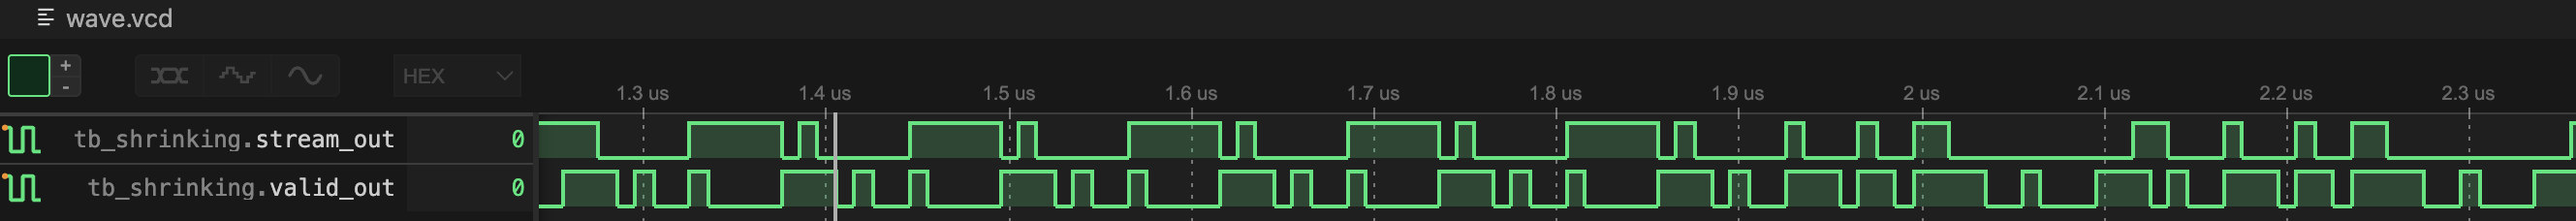
\includegraphics[width=\columnwidth]{images/LFSR1.png}}
\caption{Simulation waveform demonstrating the non-linear output of the Shrinking Generator. The \texttt{valid\_out} signal asynchronously validates the \texttt{stream\_out} data, destroying linear predictability.}
\label{fig:lfsr1}
\end{figure}

The logic operates as follows:
\begin{itemize}
    \item \textbf{LFSR A (Selector - 64-bit):} Determines whether the data bit is valid.
    \item \textbf{LFSR B (Data - 63-bit):} Generates the actual keystream bit.
\end{itemize}
If LFSR A generates a '1', the bit from LFSR B is outputted (\texttt{valid\_out = '1'}). If LFSR A generates a '0', the bit from LFSR B is discarded (shrunk), and the output state holds its previous value. This irregular decimation of the data stream entirely destroys the time-correlation of the output bits, neutralizing linear algebraic attacks.

\subsection{Mathematical Robustness and Period Maximization}
To ensure cryptographic security, the period of the pseudo-random sequence must be astronomical. This was achieved by selecting bit lengths that are coprime ($EBOB(64, 63) = 1$). 
By utilizing industry-standard \textbf{Primitive Polynomials}:
\begin{itemize}
    \item 64-bit LFSR: $x^{64} + x^4 + x^3 + x + 1$
    \item 63-bit LFSR: $x^{63} + x + 1$
\end{itemize}
The total period of the system becomes the product of their individual maximum lengths, derived from Mersenne prime theory: $(2^{64}-1) \times (2^{63}-1) \approx 2^{127}$ clock cycles.

\section{Hardware Accelerator for RSA}

RSA relies on modular exponentiation ($C = M^K \pmod N$), which involves massive numbers. Implementing this directly in hardware using standard division is prohibitively expensive in terms of silicon area and clock routing.

\subsection{The Square-and-Multiply State Machine}
The exponentiation is broken down iteratively using the Left-to-Right Binary Exponentiation algorithm. The VHDL state machine scans the key bits from the Most Significant Bit (MSB) to the Least Significant Bit (LSB). For every bit, a \texttt{SQUARE} operation is performed. If the key bit is '1', a subsequent \texttt{MULTIPLY} operation is triggered.

\begin{figure}[htbp]
\centerline{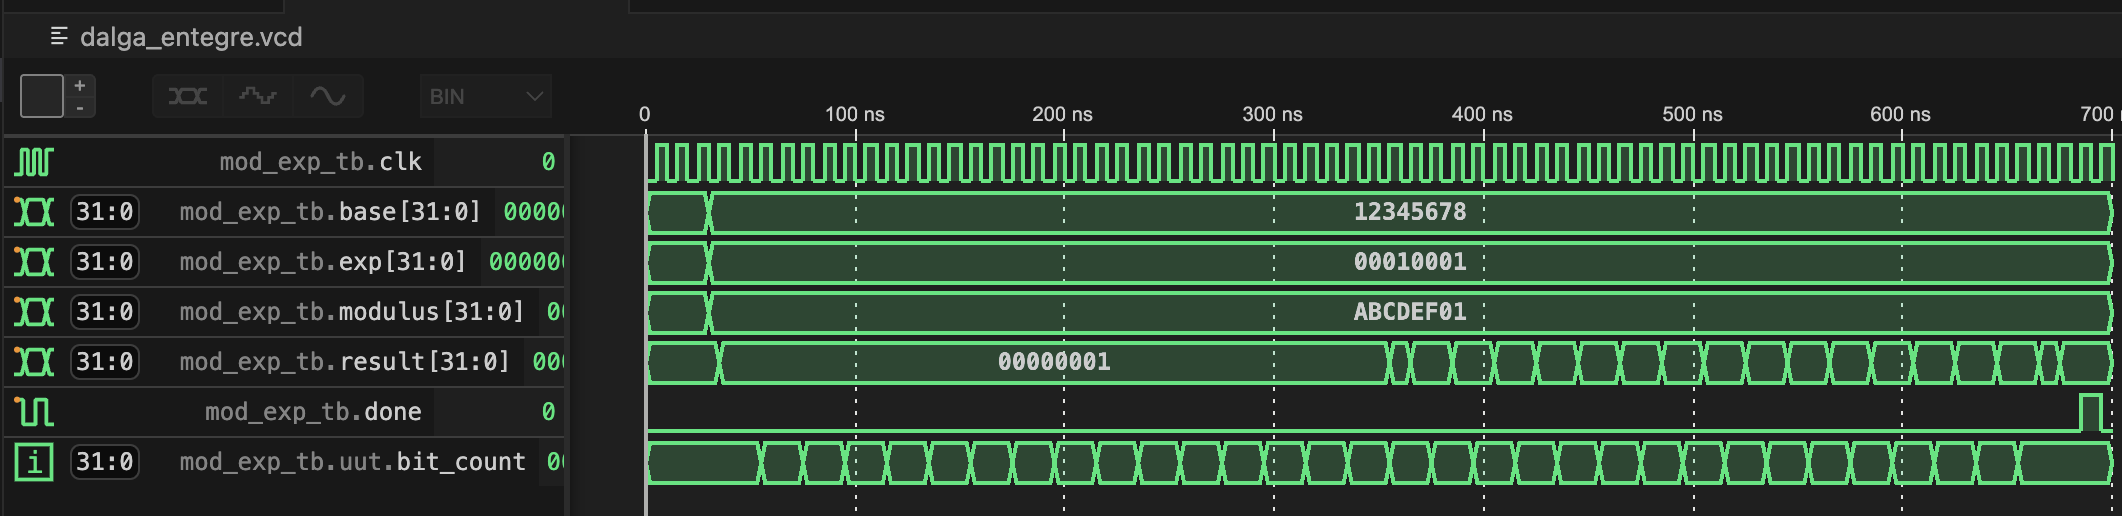
\includegraphics[width=\columnwidth]{images/RSA_engine.png}}
\caption{The Master FSM orchestrating the Square-and-Multiply loop.}
\label{fig:rsa_engine}
\end{figure}

\subsection{Montgomery Multiplication}
To execute the \texttt{SQUARE} and \texttt{MULTIPLY} operations without division, the operands are converted into the Montgomery domain. In this domain, modulo arithmetic is transformed into simple bit-shifts and additions.

\begin{figure}[htbp]
\centerline{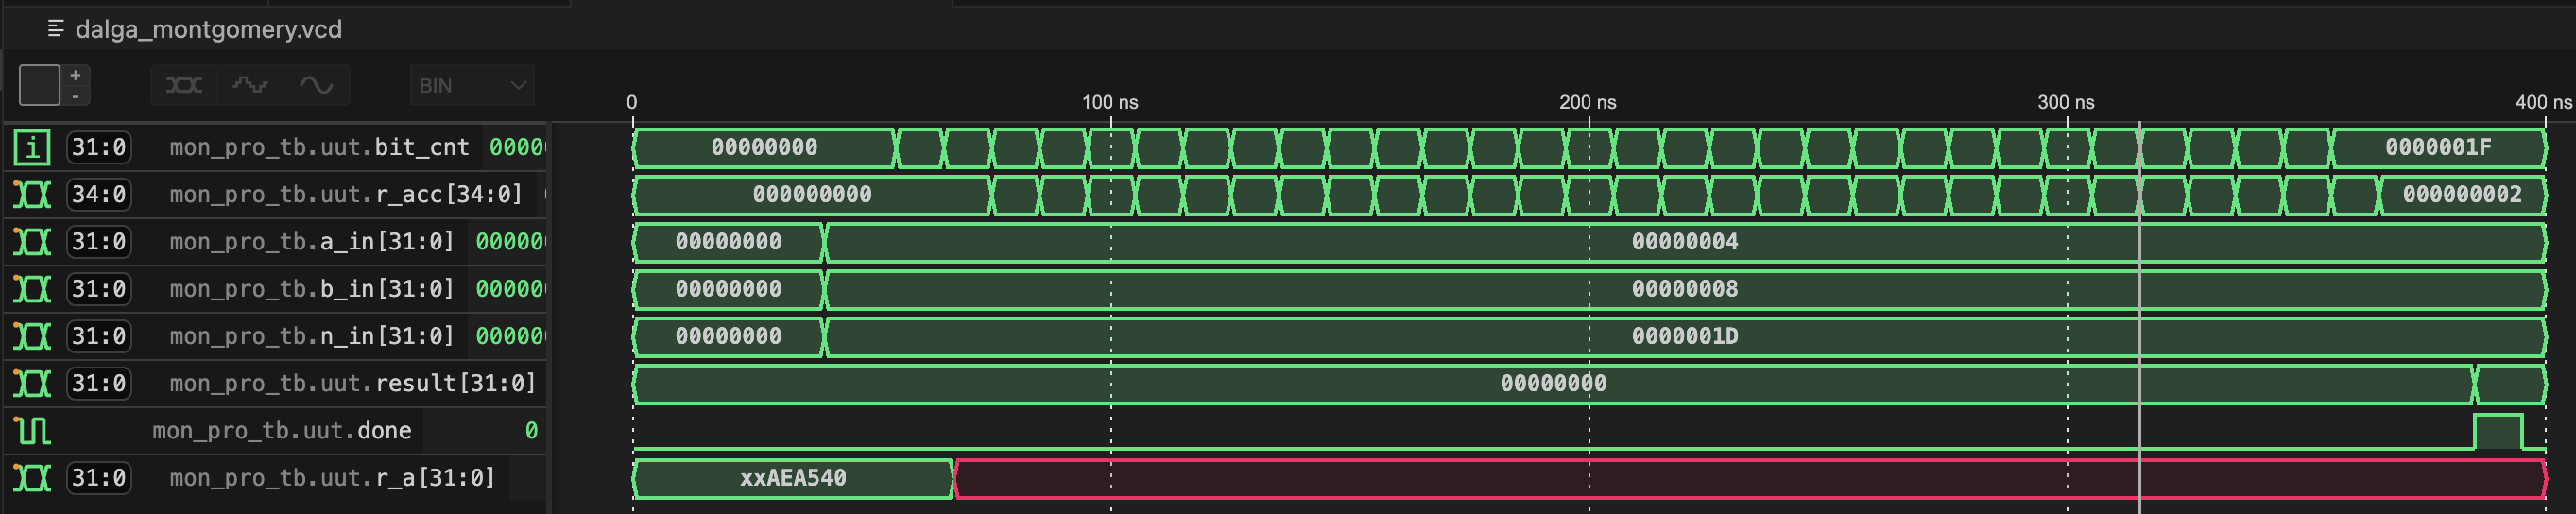
\includegraphics[width=\columnwidth]{images/RSA_montgomery.png}}
\caption{Internal waveforms of the bit-serial Montgomery Multiplier completing a multiplication cycle via consecutive additions and right-shifts.}
\label{fig:rsa_montgomery}
\end{figure}

The architecture relies on a \textbf{Master-Slave FSM}. The Master (\texttt{mod\_exp}) manages the exponent scanning and triggers the Slave (\texttt{mon\_pro}). The Slave executes the Montgomery multiplication bit-by-bit and signals a \texttt{done} flag when finished, allowing the Master to proceed.

\subsection{Results and Domain Conversion}
After the Square-and-Multiply loop completes, the final result is still in the Montgomery domain, appearing as random hex data. A final post-computation trigger converts the data back to the human-readable domain by multiplying it with $1 \pmod N$.

\begin{figure}[htbp]
\centerline{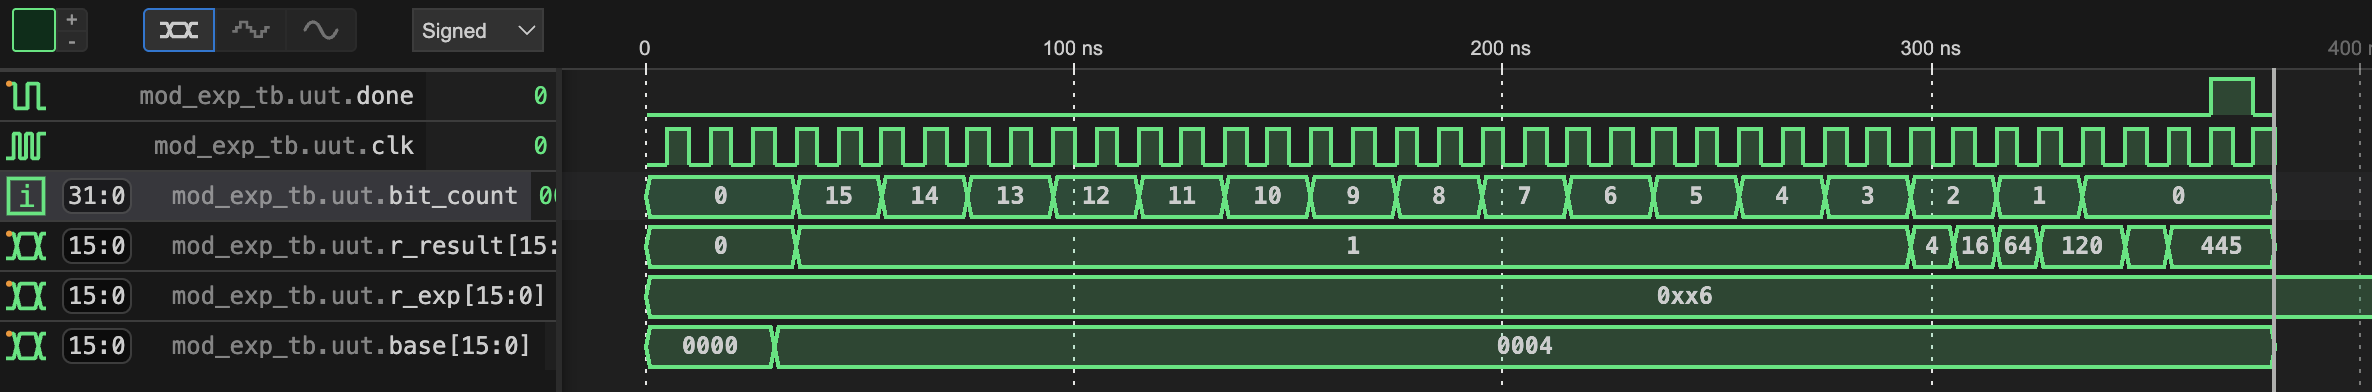
\includegraphics[width=\columnwidth]{images/RSA_16bit.png}}
\caption{Simulation of the 16-bit RSA Hardware Accelerator successfully computing the ciphertext.}
\label{fig:rsa_16bit}
\end{figure}

\begin{figure}[htbp]
\centerline{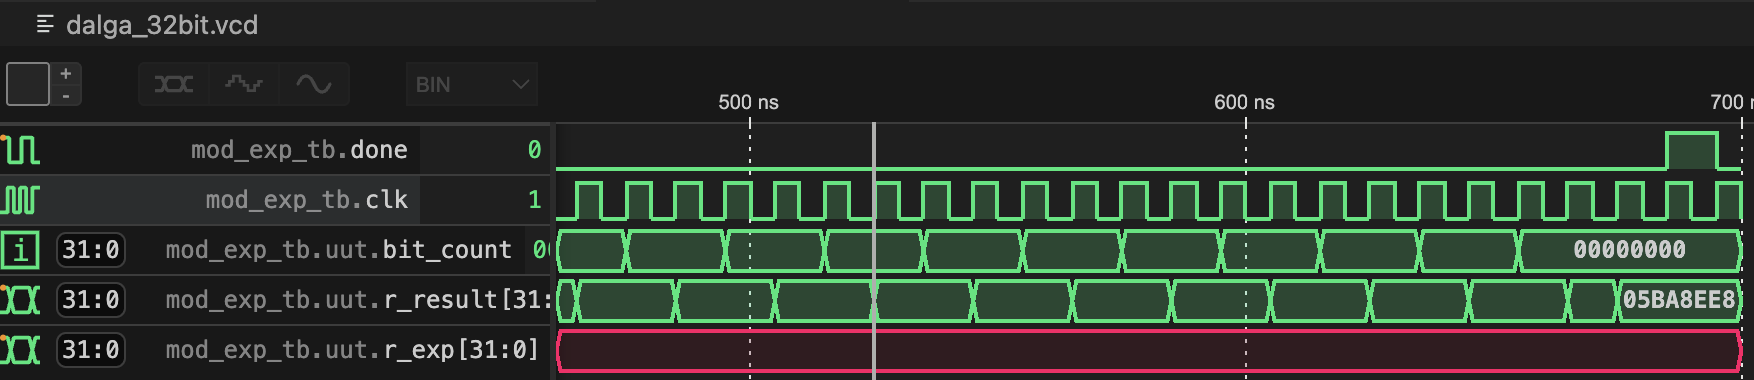
\includegraphics[width=\columnwidth]{images/RSA_32bit.png}}
\caption{Simulation of the scaled 32-bit RSA Hardware Accelerator.}
\label{fig:rsa_32bit}
\end{figure}

As shown in Figures \ref{fig:rsa_16bit} and \ref{fig:rsa_32bit}, the hardware modules successfully match standard Python cryptographic verifications for both 16-bit and 32-bit implementations.

\section{Evolution to Elliptic Curve Cryptography (ECC)}

While RSA is effective, it requires extremely large key sizes (e.g., 2048-bit) to remain secure against modern factoring attacks. Elliptic Curve Cryptography (ECC) provides the same level of security with significantly smaller keys (e.g., 256-bit), dramatically reducing silicon footprint and power consumption.

\subsection{Mathematical Foundation}
ECC operates on the algebraic structure of elliptic curves over finite fields. The standard form used in cryptography is the Weierstrass Equation:
\begin{equation}
y^2 = x^3 + ax + b \pmod p
\end{equation}

\begin{figure}[htbp]
\centerline{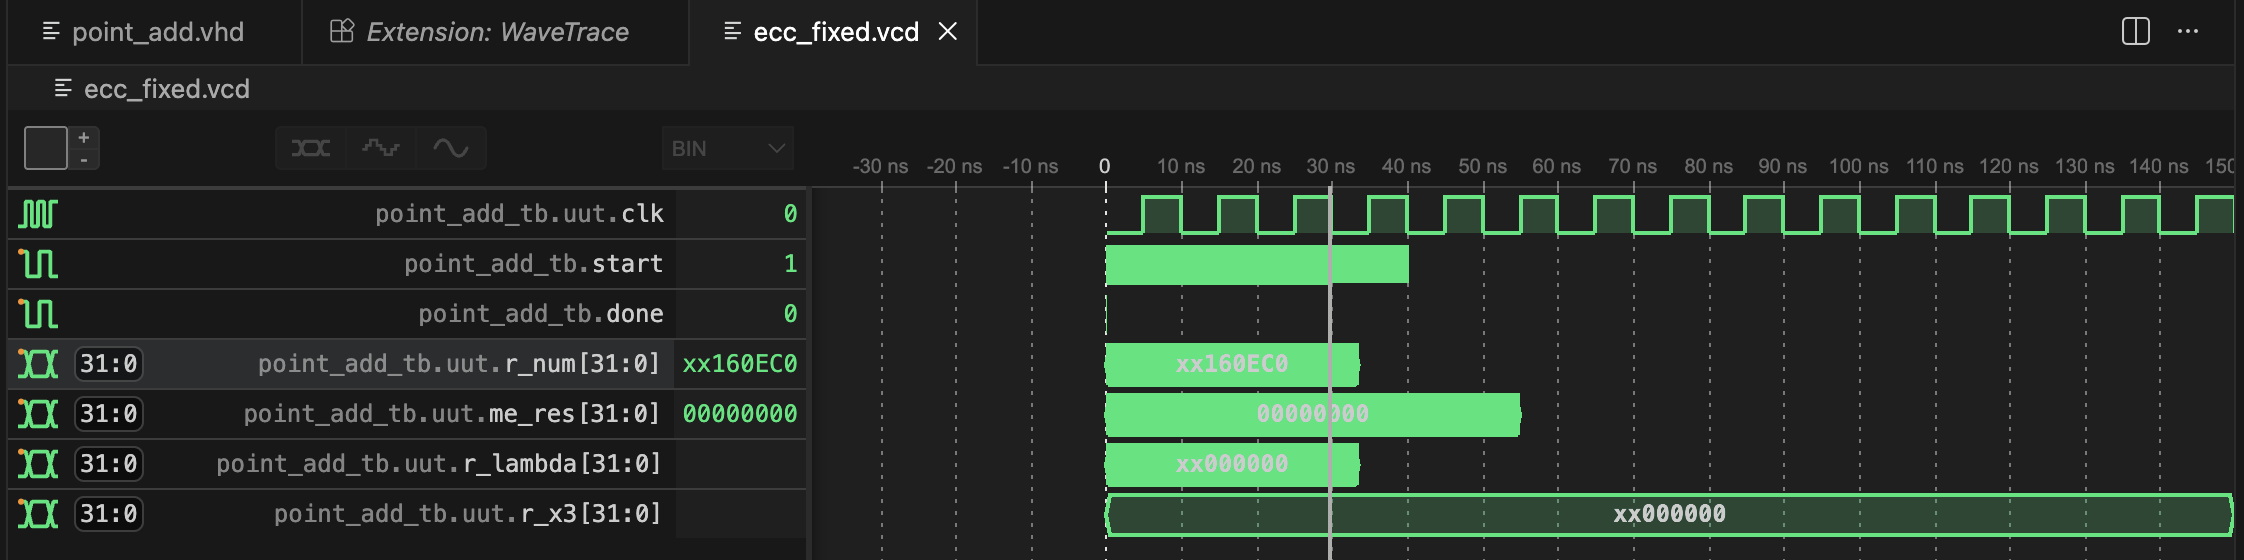
\includegraphics[width=\columnwidth]{images/ECC_starting point.png}}
\caption{A theoretical representation of an Elliptic Curve plotting points across the continuous domain.}
\label{fig:ecc_start}
\end{figure}

\subsection{Scalar Multiplication in Hardware}
The core cryptographic operation in ECC is Scalar Multiplication ($Q = kP$), where a base point $P$ is added to itself $k$ times (where $k$ is the private key). Similar to RSA's Square-and-Multiply, ECC utilizes a \textbf{Double-and-Add} algorithm.

\begin{figure}[htbp]
\centerline{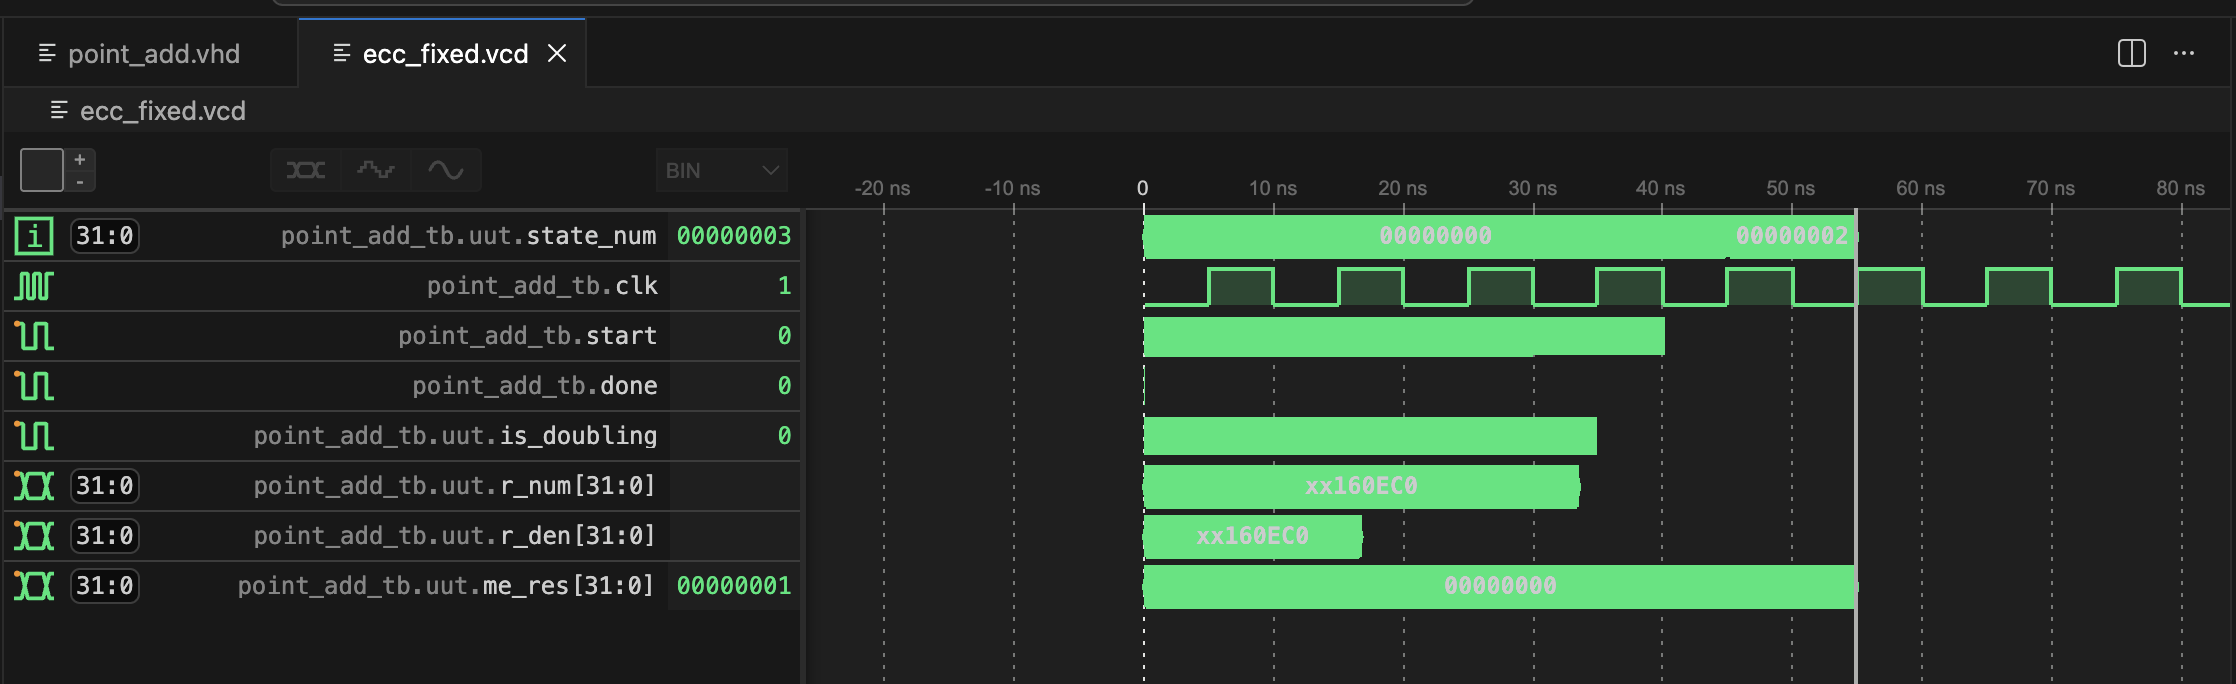
\includegraphics[width=\columnwidth]{images/ECC_point_doubling.png}}
\caption{Geometric representation of Point Doubling ($P + P = 2P$). The tangent intersects the curve, and the result is mirrored across the x-axis.}
\label{fig:ecc_double}
\end{figure}

\begin{figure}[htbp]
\centerline{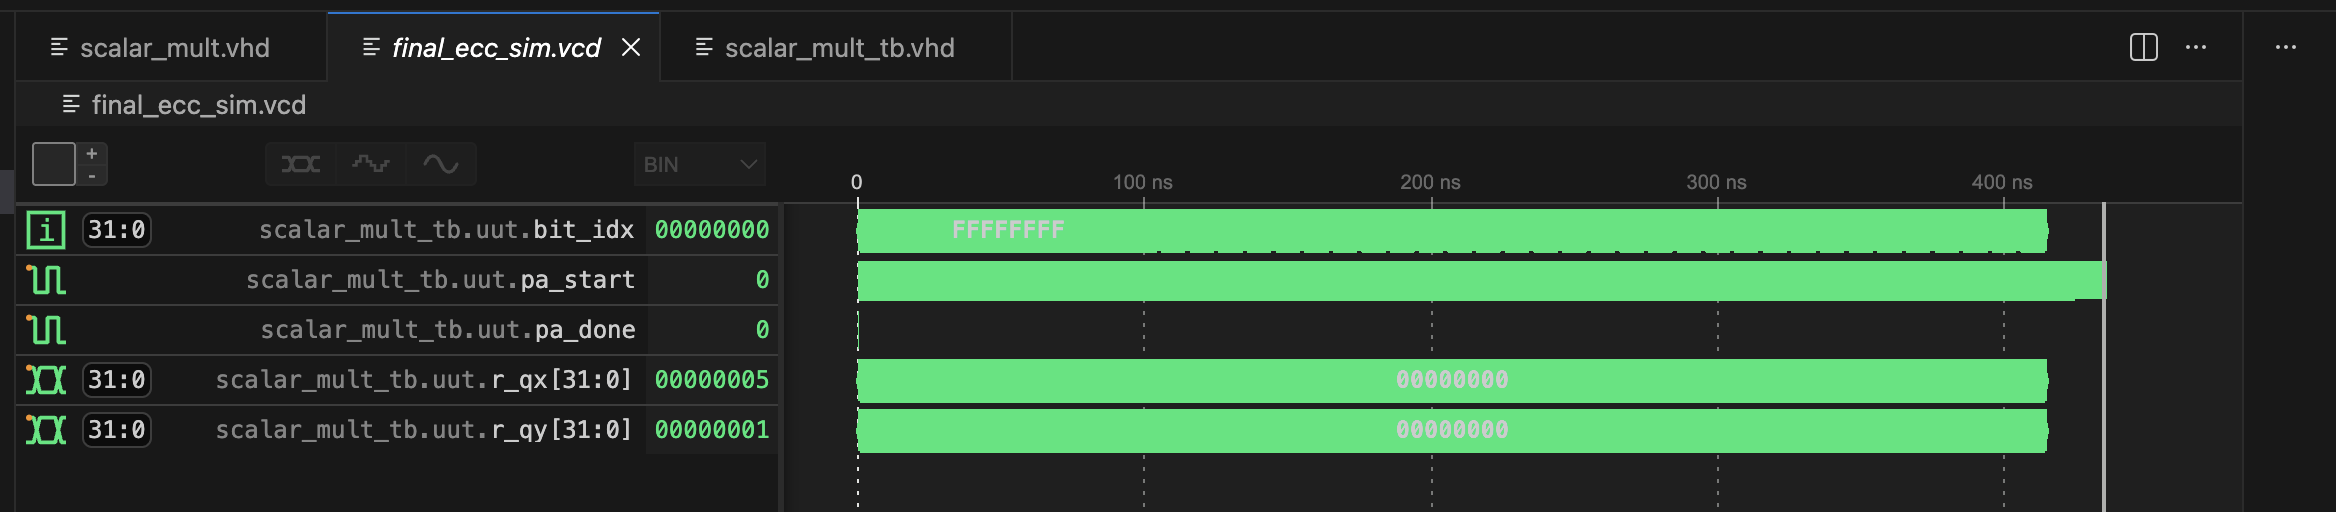
\includegraphics[width=\columnwidth]{images/ECC_Scalar_multiplication_1.png}}
\caption{Point Addition ($P + Q = R$) mechanics utilized during the "Add" phase of the algorithm.}
\label{fig:ecc_scalar1}
\end{figure}

From a hardware perspective, Point Doubling and Point Addition require entirely different sequences of modular additions, subtractions, multiplications, and inversions. Architecting an ECC engine involves designing an Arithmetic Logic Unit (ALU) capable of performing these modular operations efficiently over prime fields $GF(p)$ or binary fields $GF(2^m)$.

\section{Conclusion}
The progression from linear stream ciphers to complex public-key algorithms illustrates the incredible depth required in hardware security engineering. The Shrinking Generator successfully demonstrated how simple logical gates can establish immense cryptographic chaos. The RSA implementations showcased how mathematical algorithms like Montgomery's method can bypass the physical limitations of silicon by replacing division with shifting. Finally, the foundational exploration into Elliptic Curve Cryptography paves the way for future low-power, high-security ASIC and FPGA designs. 

\begin{thebibliography}{00}
\bibitem{b1} W. Meier and O. Staffelbach, ``The Shrinking Generator,'' \emph{Advances in Cryptology — CRYPTO '93}, Springer, 1993, pp. 205--214.
\bibitem{b2} P. L. Montgomery, ``Modular Multiplication Without Trial Division,'' \emph{Mathematics of Computation}, vol. 44, no. 170, pp. 519--521, 1985.
\bibitem{b3} N. Koblitz, ``Elliptic curve cryptosystems,'' \emph{Mathematics of Computation}, vol. 48, no. 177, pp. 203--209, 1987.
\end{thebibliography}

\end{document}
